\documentclass{article}
\usepackage{graphics}
\usepackage{graphicx}
\usepackage[T1]{fontenc}
\usepackage{float}
\usepackage[margin=1in]{geometry}
\usepackage[utf8]{inputenc}

\DeclareGraphicsExtensions{.eps}


\title{CS 742 Foundations of Network Security and Cryptography \\ Assignment 3}
\author{
  Ajay Kedare \\
  153059007
  \and
  Astha Jada \\
  153050027
  \and
  Neha Garg \\
  153050039
  \and
  Sankalp Rangare \\
  153050087
}

\date{}

\begin{document}
\maketitle
\clearpage


\section{Re-design the Needham-Schroeder protocol to use as few messages as possible. Prove
informally that your protocol is secure.
If you could use timestamps in lieu of ( or in addition to nonces), what is the smallest
number of messages you need to achieve the same functionality provided by the
Needham-Schroeder protocol? Show your new design.}

 \begin{enumerate}
  \item $A \rightarrow B: M,A,B,\{N_a,M,A,B \}K_{as}$
  \item	$B \rightarrow KDC: M,A,B,\{N_a,M,A,B \}K_{as}, \{N_b,M,A,B\}K_{bs}$
  \item $KDC \rightarrow B: \{M,N_a,K_{a,b}\}K_{as},  \{M,N_b,K_{a,b}\}K_{bs}$
  \item $B \rightarrow A: \{N_a,K_{a,b}\}K_{as} , \{N_b\}K_{ab}$
  \item $A \rightarrow B: \{N_b-1\}K_{ab}$
 \end{enumerate} 
 
 \noindent Here, M is session identifier. \\ 
 \indent $N_a and N_b$ are the nonces. \\ \\
 
 \noindent $A \rightarrow B: M,A,B,\{N_a,M,A,B \}K_{as}$ \\
 A sends encrypted data to KDC which includes nonce,session identifier and identities of A \& B. A also sends this in plaintext to B. \\ \\ 
 $B \rightarrow KDC: M,A,B,\{N_a,M,A,B \}K_{as}, \{N_b,M,A,B\}K_{bs}$ \\ 
 B now communicates with KDC and forwards A's encypted data along with encrypted data from B which includes B's nonce, session idenitifier and identities of A \& B. \\ \\
 $KDC \rightarrow B: \{M,N_a,K_{a,b}\}K_{as},  \{M,N_b,K_{a,b}\}K_{bs}$\\
 KDC, replies back with session key $K_{ab}$ for both A \& B which is encrypted with shared keys of A \& B with KDC. \\ \\
 $B \rightarrow A: \{N_a,K_{a,b}\}K_{as} , \{N_b\}K_{ab}$\\
 B sends the received ticket to A which has session key and also nonces encrypted with session key. \\ \\
 $A \rightarrow B: \{N_b\}K_{ab}$ \\
 A decrypts the session key from ticket and verifies the nonces by using session key. \\ \\ 
 
 This protocol provides key confirmation and entity authentication. A is sending nonce to B which is encrypted for KDC, and when A recieves back the session key, it verifies the nonce with the nonce earlier sent to KDC. Hence any replay of message will be detected with the freshness of nonce.
 
 
    
\vspace{1cm}
\noindent Using timestamp we reduced the number of messages to 4 as below: \\
 \begin{enumerate}
  \item $A \rightarrow B: A,N_a$
  \item	$B \rightarrow KDC: B,N_b,\{A,N_a,T_b\}K_{bs}$
  \item $KDC \rightarrow A: \{B,N_a,K_{ab},T_b\}K_{as}, \{A,K_{ab},T_b\}K_{bs},N_b$
  \item $A \rightarrow B: \{A,K_{ab},T_b\}K_{bs}, \{N_b\}K_{ab}$
 \end{enumerate} 
 
 \noindent Here, $T_b$ is timestamp which specifies the duration for which session is valid. \\ 
 \indent $N_a and N_b$ are the nonces. \\
 
 
 \noindent 
 $A \rightarrow B: A,N_a$ \\ First, A sends his identification and nonce to B.\\ \\
 $B \rightarrow KDC: B,N_b,\{A,N_a,T_b\}K_{bs}$\\ B forwards this nonce and A's identification to KDC requesting for the ticket.
 which is encrypted with $K_{bs}$. B also sends his nonce so that he can verify when he recives the actual session key. 
 A timestamp is added that decides the duration of session. \\ \\
 $KDC \rightarrow A: \{B,N_a,K_{ab},T_b\}K_{as}, \{A,K_{ab},T_b\}K_{bs},N_b$ \\
 KDC, now generates the session key $K_{ab}$ and forward it to A along with A's nonce, timestamp $T_b$ encrypted with $K_{as}$.
 It also includes the ticket which has the session key, timestamp and will be forwarded to B. \\ \\
 $A \rightarrow B: \{A,K_{ab},T_b\}K_{bs}, \{N_b\}K_{ab}$ \\
 A forwards the ticket to B which has session key,timestamp and enrypts the B's nonce with session key $K_{ab}$ \\
 
 
 Here B recieves the ticket from A and will verify the timestamp whether the ticket is valid for that duration or not hence any replay attack is not possible which is outside the valid duration.
 

 
 

 
\section{Study the following attacks on SSL or on OpenSSL – BEAST, Heartbleed, Fluke. For each
attack answer the following:
What does the attack accomplish?
Desribe a “typical” attack scenario.
What is the vulnerability behind the attack?
How can the attack be defended against?}

\subsection{Beast}
\subsubsection{What does the attack accomplish?}

\indent \indent BEAST Attack which stands for {\it Browser Exploit Against SSL/TLS Attack} is based on "chosen plain text attack". TLS 1.0 uses CBC (Cipher Block Chaining) mode of operation for encryption. CBC modes makes use of previous cipher text block  $C_{i-1}$ as the initialization vector (IV) for encrypting the next plain text block $P_{i}$.

If an attacker is sniffing the encrypted data sent by the browser, then he/she will be able to obtain the IV that will be used for the next message encyption. So if the attacker can make a guess at the session cookie ($P_{i}$) and see if this new  cipher text ($C'_{i}$)
matches with original cipher text ($C_{i}$) then attacker has made a correct guess at the session cookie.

\subsubsection{Desribe a “typical” attack scenario.}
\indent \indent Considering that attacker has identified a  block of ciphertext Ci that he/she wants to decrypt, becuase it contains the session cookie. Now as he already sinffed the network so he already has Ci-1 with him.
As per CBC mode of operation: $C_i=Ek(P_i \oplus C_{i-1})$
Attacker will write a Javascript program to transmit any chosen plain text block $P_i$ that he/she wants to encrypt. Then it will produce a ciphertext $C'_i$ that attacker can sniff.
Suppose attacker has correctly guessed the plain text $P_i$ then attacker will generate $P'_i= IV \oplus P_i \oplus C_{i-1}$. Now with the help of the javascript which attacker has created he will force $P_i$ to be replaced with $P'_i$. Now TLS layer will encrypt it as: \\ 

\noindent $C'_i = Ek(IV \oplus P'_i)$ \\
After putting $P'_i$ value we'll get \\ 
$C'_i = Ek(IV \oplus IV \oplus P_i \oplus C_{i-1}) $\\ 
IV $\oplus$ IV will cancel out each other we will get\\
$C'_i = Ek(P_i \oplus C_{i-1})$ \\
If this $C'_i$ is identical to $C_i$ we can conclude that attacker has correctly guess the plain text block $P_i$. If they are not identical then attacker needs to guess the plain text block untill he/she finds a match.

\subsubsection{What is the vulnerability behind the attack?}
\indent \indent As TLS 1.0 uses CBC (Cipher Block Chaining) mode of operation for encryption. CBC modes makes use of previous cipher text block $C_{i-1}$ as the initialization vector (IV) for encrypting the next plain text block $P_i$.

\subsubsection{How can the attack be defended against?}
\indent \indent This attack can be avoided by instead of directly using previous cipher text block as IV we can have explicit IV for each block to be encypted. This attack was addressed in TLS 1.1 and TLS 1.2 by the use of “explicit IVs” for each block.

\subsection{Heartbleed}

\indent \indent OpenSSL versions 1.0.1 through 1.0.1f (inclusive) are vulnerable to the heartbleed attack.
In SSL when client communicates to the server it regularly sends heartbeat messages to the server to see if the server is alive. If the server is alive it sends reply back to the client. Both server and client sends out messages regularly to make sure both the parties are alive. This feature is used in the heartbleed attack.

The heartbeat message consists of a payload, typically a text string, along with the payload's length as a 16-bit integer. The receiving computer then must send exactly the same payload back to the sender. The vulnerable versions of OpenSSL allocate a memory buffer for the message to be returned based on the length field in the requesting message, without checking the actual size of that message's payload. As proper bound checking is not done the message returned consists of the payload, possibly followed by whatever else happened to be in the allocated memory buffer.

\subsubsection{What does the attack accomplish?}
\indent \indent Heartbleed is therefore exploited by sending a malformed heartbeat request with a small payload and large length field to the vulnerable party permitting attackers to read up to 64 kilobytes of the victim's memory.Attackers in this way could receive sensitive data, compromising the confidentiality of the victim's communications like username,passwords etc. The worse thing is that sometimes the private key can also be exposed and the attacker which would enable attackers to decrypt communications.

\subsubsection{Desribe a “typical” attack scenario.}
\indent \indent A Heartbeat Request might ask a party to "send back the three-letter word 'abc'", resulting in a response of "abc" while a  malicious heartbeat request of "send back the 500-letter word 'abc'" would cause the victim to return "abc" followed by whatever 497 characters the victim happened to have in active memory.As described above this may cause the victim to send sensitive data to the attacker.

\subsubsection{What is the vulnerability behind the attack?}
\indent \indent The vulnerability of this attack lies in the OpenSSL implementation. Here the receiver of heartbeat message does not check the bounds i.e if the length is same as the message received.


\subsubsection{How can the attack be defended against?}
\indent \indent The attack can be defended by doing proper bound checking. Also if the private key is compromised it should be revoked and new private key should be used, else the attacker may decrypt the message or can also change the message.

\subsection{Freak}
\indent \indent FREAK (Factoring RSA Export Keys) is a security exploit of a cryptographic weakness in the SSL/TLS protocols.The vulnerability was introduced during 1990's, when the US government banned selling strong cryptographic software overseas, unless it used export cipher suites which involved encryption keys no longer than 512-bits so it can be decrypted by NSA.

The need to support export cipher suites led to some technical challenges. Since U.S. servers needed to support both strong and weak cryptographic algorithms, the SSL designers used a 'cipher suite' negotiation mechanism to identify the best cipher both parties could support. As a result the strong cipher can be used when available and weaker otherwise.

\subsubsection{What does the attack accomplish?}
\indent \indent Using this attack an attacker can impersonate as the client and exchange messages with the server. The message can also be modified by the attacker.

\subsubsection{Desribe a “typical” attack scenario.}
\indent \indent FREAK attack basically is a  Man in the Middle(MITM) attack that uses export cipher suite. The attack can be done as follows: \\
\begin{enumerate}
 \item The client asks the server for the standard 'RSA' ciphersuite.
 \item The MITM attacker changes this message and asks for 'export RSA'.
 \item The server then responds with a 512-bit export RSA key, signed with its long-term key.
 \item The client accepts this weak key due to the bug in OpenSSL implementation.
 \item The attacker factors the RSA modulus to recover the corresponding RSA decryption key.
 \item When the client encrypts the 'pre-master secret' to the server, the attacker can now decrypt it to recover the 'master secret'.
 \item From here on, the attacker sees plaintext and can inject anything it wants.
\end{enumerate}

\subsubsection{What is the vulnerability behind the attack?}
\indent \indent The vulnerability behind this attack is that export cipher suites are still supported by some of the servers and they can be easily decrypted.

\subsubsection{How can the attack be defended against?}
\indent \indent The server should disable support for any export suites. Administrators should be encouraged to disable all insecure ciphers and enable suites which support perfect forward secrecy i.e if a session key is revealed it should not affect the future messages and they cannot be decrypted.

\section{Buffer overflow vulnerability}
  \subsection{On linux machine(x86\_64)}
  We completed buffer overflow attack using  x=56 and y=7.\\
        
  \noindent 1. We disabled canary variable and make Stack executable and compiled program using:\\
  \textbf{\tt gcc -g -fno-stack-protector -z execstack -o prog prog.c}\\\\
  2. Now we started to debug the program using \textbf{gdb}.\\
    We added a break point in function \textbf{A( )} and analysed the program.\\
    We checked the address of local varibales of function \textbf{A( )}.\\
  
  \begin{figure}[htb]
   \begin{center}
		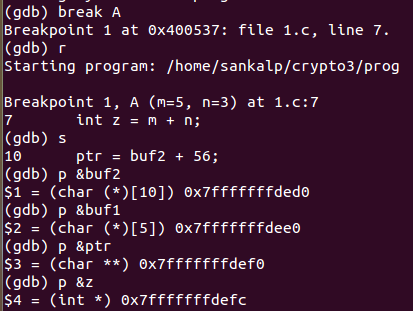
\includegraphics[width=8cm,height=5cm]{bo.png}
	\caption{Address of local varibales.}
	 \end{center}
	\end{figure}
      After getting the address of local variables we 'disassemble' the main function
      and checked the return address of function \textbf{A( )}.\\
      
       
   
   \begin{figure}[htb]
     \begin{center}
		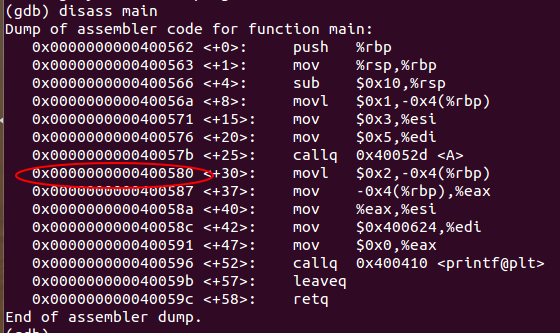
\includegraphics[width=8cm,height=4cm]{bo1.png}
	\caption{Return address of function A()}
	 \end{center}
	\end{figure}
        

    3.Stack layout:    
         \begin{figure}[H]
            \begin{center}
		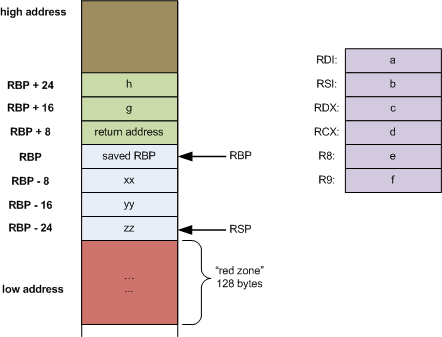
\includegraphics[width=8cm,height=8cm]{stack.png}
	\caption{Stack frame layout}
	  \end{center}
	\end{figure}
        
        As we can see in stack frame return address is stotred in (base-pointer+8) address.\\
        We check the content of registers and get the address of base-pointer stored in register \textbf{rbp}.\\
         
         \begin{figure}[H]
          \begin{center}
		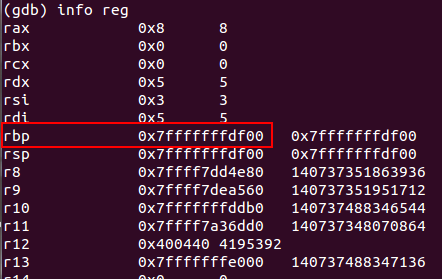
\includegraphics[width=8cm,height=8cm]{reg.png}
	\caption{Base-pointer address}
	\end{center}
	\end{figure}
         
         (base-pointer address + 8) will give the location where return address is stored.\\
          
           \begin{figure}[H]
             \begin{center}
		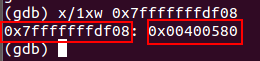
\includegraphics[width=8cm,height=2cm]{ret.png}
	\caption{Location of return address in stack-frame}
	\end{center}
	\end{figure}
         
         Now,we have the location of \textbf{return address} and address of buf2.\\
         We calculated the differnce between these two
         addresses,which will give value of \textbf{x=56.}\\
         As we can see from the assembly code of main function,next address after the return address of \textbf{A()} is \textbf{0x400587}.\\
          So we change the return address by adding \textbf{7} to the content of \textbf{*ptr} variable.\\
          Therefore value of \textbf{y=7.}\\
          
          Similarly when canary varibale is enabled,we get different values \textbf{x=40 and y=7}.\\
          In this case values are different because compiler does some optimization on allocation of local variables\\
           in the stack and compiler allocate memory in different manner and also canary variable is also in the stack.\\
           
           \begin{figure}[H]
             \begin{center}
		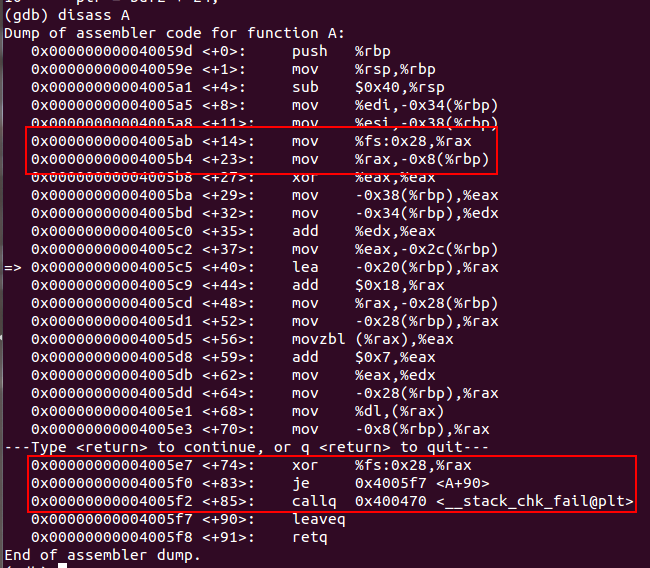
\includegraphics[width=8cm,height=8cm]{can.png}
	\caption{Canary varibale intialization and checking for buffer-overflow attack}
	\end{center}
	\end{figure}
         
 \subsection{On Windows(x86\_64)}
  \subsubsection{Canary variable is enabled}
  
  1. On windows machine stack word size is 4 bytes.
      
      \begin{figure}[H]
	\begin{center}
	 

 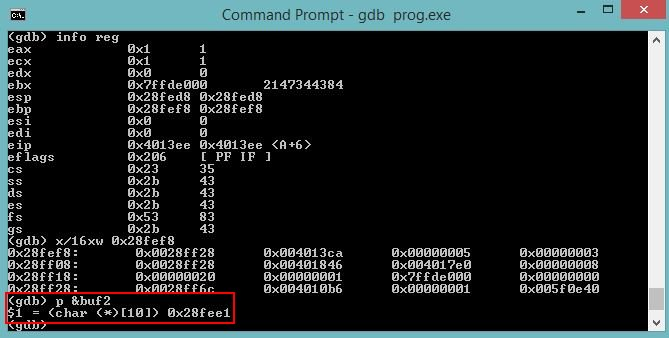
\includegraphics[width=8cm,height=8cm]{buf2addr.JPG}
	\caption{Address of buf2}
		\end{center}
	\end{figure}
  2. We now check for return address of function A.
       
       
      \begin{figure}[H]
       \begin{center}
		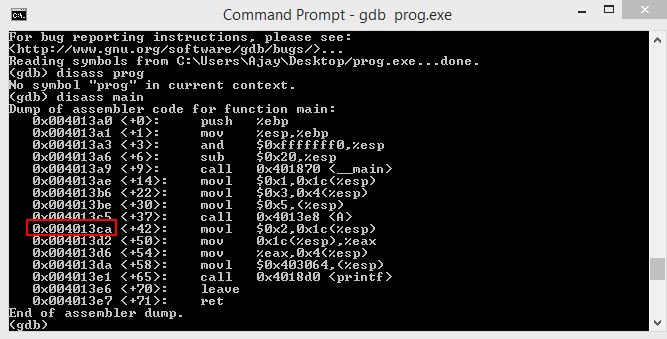
\includegraphics[width=8cm,height=8cm]{disassMain.JPG}
	\caption{Return address of function A}
	\end{center}
	\end{figure}
  3. Checking contents of register to get address of base-pointer of stack-frame of function A.\\
   
      \begin{figure}[H]
           \begin{center}
		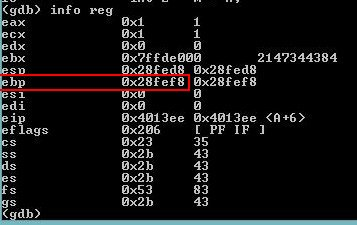
\includegraphics[width=8cm,height=8cm]{infoReg.JPG}
	\caption{Address of base-pointer}
	\end{center}
	\end{figure}
     
     (base-pointer +4) will give the location of return Address stored in stack frame.\\
     So,\textbf{ox28fefc} is the location where return address is stored.\\
     Therefore value of x=27(differnce between location of return address and address of buf2)\\
     And value of y=8.\\
    
   \subsubsection{Canary variable is disabled}
   \indent To disable the canary in windows machine we compile our program with command as : \\
   \textbf{\tt gcc -g -fstack-protector -o prog prog.c}\\\\
   Similarly with stack-protection on we get \textbf{x=26 and y=8.}\\
   This is because memory for local variables are allocated differently in presence of canary variable.\\
    
    \begin{figure}[H]
             \begin{center}
		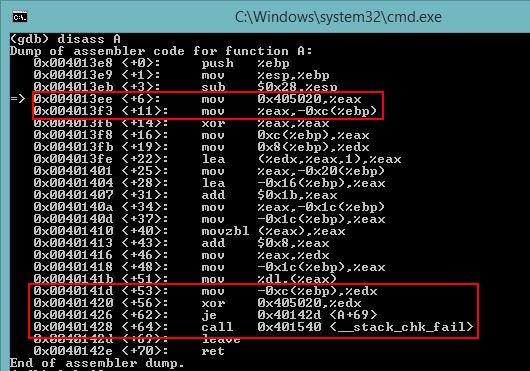
\includegraphics[width=8cm,height=8cm]{ws.JPG}
	\caption{Canary varibale intialization and checking for buffer-overflow attack}
	\end{center}
	\end{figure}
  
  \begin{table}[H]
\centering
\caption{Values of x and y}
\label{my-label}
\begin{tabular}{|l|l|l|}
\hline
\begin{tabular}[c]{@{}l@{}}linux(x\_86\_64)\\ canary disabled\end{tabular}   & x=56 & y=7 \\ \hline
\begin{tabular}[c]{@{}l@{}}linux(x\_86\_64)\\ canary enabled\end{tabular}    & x=40 & y=7 \\ \hline
\begin{tabular}[c]{@{}l@{}}windows(x\_86\_64)\\ canary disabled\end{tabular} & x=27 & y=8 \\ \hline
\begin{tabular}[c]{@{}l@{}}windows(x\_86\_64)\\ canary enabled\end{tabular}  & x=26 & y=8 \\ \hline
\end{tabular}
\end{table}

\end{document}

